\documentclass[tikz,border=8pt]{standalone}
\usetikzlibrary{arrows.meta,backgrounds,fit,positioning}

\definecolor{systemblue}{HTML}{D9EAF7}
\definecolor{systemgreen}{HTML}{D9EAD3}
\definecolor{systemyellow}{HTML}{FFF2CC}
\definecolor{systemgray}{HTML}{F2F2F2}
\definecolor{systemline}{HTML}{4F6D7A}

\tikzset{
  flowbox/.style={
    draw=systemline,
    rounded corners=2pt,
    fill=#1,
    minimum width=3.15cm,
    minimum height=1.05cm,
    align=center,
    font=\sffamily\small
  },
  flowbox/.default=systemgray,
  store/.style={
    draw=systemline,
    rounded corners=2pt,
    fill=systemyellow,
    minimum width=2.6cm,
    minimum height=1.0cm,
    align=center,
    font=\sffamily\small
  },
  arrow/.style={-Latex,thick,draw=systemline},
  group/.style={draw=systemline,rounded corners=4pt,dashed,inner sep=8pt}
}

\begin{document}
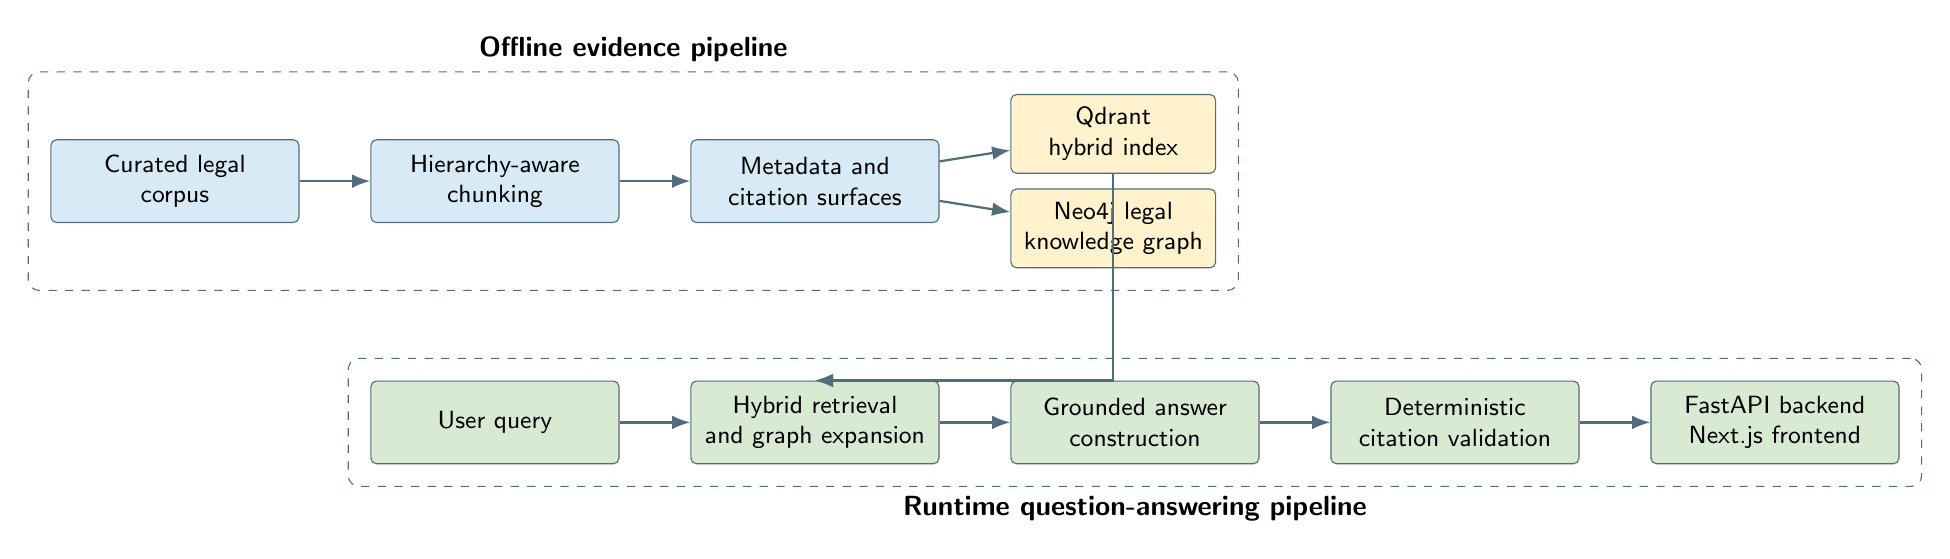
\begin{tikzpicture}[node distance=0.75cm and 0.9cm]
  \node[flowbox=systemblue] (corpus) {Curated legal\\corpus};
  \node[flowbox=systemblue, right=of corpus] (chunk) {Hierarchy-aware\\chunking};
  \node[flowbox=systemblue, right=of chunk] (enrich) {Metadata and\\citation surfaces};
  \node[store, right=of enrich, yshift=0.6cm] (qdrant) {Qdrant\\hybrid index};
  \node[store, right=of enrich, yshift=-0.6cm] (neo4j) {Neo4j legal\\knowledge graph};

  \node[flowbox=systemgreen, below=2.0cm of chunk] (query) {User query};
  \node[flowbox=systemgreen, right=of query] (retrieve) {Hybrid retrieval\\and graph expansion};
  \node[flowbox=systemgreen, right=of retrieve] (answer) {Grounded answer\\construction};
  \node[flowbox=systemgreen, right=of answer] (validate) {Deterministic\\citation validation};
  \node[flowbox=systemgreen, right=of validate] (frontend) {FastAPI backend\\Next.js frontend};

  \draw[arrow] (corpus) -- (chunk);
  \draw[arrow] (chunk) -- (enrich);
  \draw[arrow] (enrich) -- (qdrant);
  \draw[arrow] (enrich) -- (neo4j);
  \draw[arrow] (query) -- (retrieve);
  \draw[arrow] (retrieve) -- (answer);
  \draw[arrow] (answer) -- (validate);
  \draw[arrow] (validate) -- (frontend);
  \draw[arrow] (qdrant.south) |- (retrieve.north);
  \draw[arrow] (neo4j.south) |- (retrieve.north);

  \begin{scope}[on background layer]
    \node[group,fit=(corpus)(chunk)(enrich)(qdrant)(neo4j),label={[font=\sffamily\bfseries]above:Offline evidence pipeline}] {};
    \node[group,fit=(query)(retrieve)(answer)(validate)(frontend),label={[font=\sffamily\bfseries]below:Runtime question-answering pipeline}] {};
  \end{scope}
\end{tikzpicture}
\end{document}
